\documentclass[nochapterpage,bigchapter,linedtoc,longdoc,colorback,accentcolor=tud3b,oneside]{tudreport}

\usepackage[stable]{footmisc}
\usepackage[ngerman]{hyperref}

\usepackage{longtable}
\usepackage{multirow}
\usepackage{booktabs}

\hypersetup{%
  pdftitle={Making Matches - Recommending the right personality
  },
  pdfauthor={Paul Schweiger},
  pdfsubject={Personality Recommendation},
  pdfview=FitH,
  pdfstartview=FitV
}

\newlength{\longtablewidth}
\setlength{\longtablewidth}{0.7\linewidth}
\addtolength{\longtablewidth}{-\marginparsep}
\addtolength{\longtablewidth}{-\marginparwidth}

\graphicspath{{g/}}

\title{Making Matches - Recommending the right personality}
\subtitle{Paul Schweiger}

\begin{document}
\maketitle


\chapter{Quick note for reviewers}
As you probably know, Latex likes to screw around. It is now 30 minutes before I have to hand in this report for you to review it, and Latex decided 20 minutes ago to completely destroy all of my citations. The control sequences returns as undefined, and I can't figure out how to fix this. Since I totally did NOT want to remove all citations, the easiest way to force this file to compile was to exchange the cite command to an italic command, meaning that all those weird bibtex references you will see in the text are supposed to look good, but don't.\\
Im sorry for any inconvenience, as I am aware that this makes reading harder. Additionally, my references will not be included in this version of the report. [But, tbh, nobody would have looked at them anyway, right?]\\
Thank you very much, and have "fun" reading this report ;)


\chapter{Introduction}
The modern world provides a plethora of opportunities, topics, people, products, and other things, while people have a limited amount of attention and time to spend. In order to help us guide our attention and resources, basically every digital product tries to recommend meaningful content to users. Recommender Systems play a critical role in modern society and have transcended in many different domains, pervading our lifes in advertising, e-learning, online-dating, video game matchmaking, social networks, e-commerce, data analysis, and many other topics.\\
As the offline world embraces online opportunities, a surplus of possible social contacts emerges, making it challenging to engage with the right person at the right time.\\
Social contacts are highly important in many domains, but form a cornerstone in furthering educational goals.\\
Social and cooperative learning are generally seen as positively affecting learning outcomes. \textit{bossert1982instructional, blumenfeld1996learning} Successful group learning efforts can enhance cognitive and intellectual performance, student's social and communication skills and influence their overall satisfaction. \textit{zhao2004adding, maxwell2008learning}\\
The focal point of technology-enhanced educational research is to improve the individual learning experiences of students by recommending them exercises, media resources and additional information at the right time, depending on the student's skills, preferences, needs and personality. \textit{drachsler2015panorama, erdt2015evaluating} In social contexts, opportunities for students to receive immediate peer support via online requests have been explored, \textit{greer1998intelligent} or students tasked to discuss their answers to questions in an E-learning environment with their peers leading to improvements in both short- and long-term performance. \textit{reidsema2016exploring}\\
The goal of this report is to emphasize how Recommender Systems can be used not only to help a single learner to solve problems or improve learning results, but to connect people, to build a community of learners and to enable students to engage in meaningful social learning opportunities. Along the way, relevant examples from other domains will be featured. We will take a look at the basics of user modeling in section \ref{rw:usermodeling}, social recommendations in section \ref{rw:socialrec} and the importance of reciprocality in section \ref{rw:reciprocalrec}. Chapter \ref{paper} will highlight the intricacies of learning group formation and evaluate a recent prototype for reciprocal peer recommendation for learning purposes.\\

%remove whitespace after chapter start
\renewcommand{\cleardoublepage}{}
\renewcommand{\clearpage}{}


\chapter{Related Work: Recommender Systems}

\section{User Modeling} \label{rw:usermodeling}
The goal of a Recommender System [RS] is to emphasize relevant pieces of information in a convoluted stream of data, and to recommend a specific result to a specific user based on his or her history, preferences and situation. \textit{ricci2011introduction}\\
In order to successfully recommend items, an RS needs to understand it's user. The goals, circumstances and domain-specific aspects need to be considered. Thus, RS need to model their users to try and understand what items might be fitting. Recommender Systems need account for an adequate operationalization of the relevant personality traits, domain-specific skills and surrounding circumstances.\\
Different domains or approaches within the same domain require different user models. For example, information about people connected to the current user can be helpful to improve recommendation quality. Based on user friendships and shared interests, specific items that one person liked could be recommended to friends \textit{feng2013recommendation} or just other users with comparable interests. \textit{hsu2018general} Another approach used to enable recommendations with scarce data and mobile computing power was to access a user's contacts and geographic history to find users with matching profiles and more information that can be used to improve recommendations. \textit{ramaswamy2009caesar}\\ 
Even within a single domain, for example multiplayer videogame matchmaking, a system could focus on self-reported preferences \textit{riegelsberger2007personality}, ratings by other players \textit{patrick2011system}, implicit gameplay-derived data \textit{suznjevic2015application, delalleau2012beyond} or a combination of technical and self-reported information to improve the overall gaming experience. \textit{farnham2009method}\\
A recent study by Wang et al. \textit{wang2015thinking} for example looked at the enjoyment of multiplayer gaming sessions in League of Legends (LoL) based on player personality. They followed a subset of Sternberg's \textit{sternberg1999thinking} problem-solving styles in order to categorize the playstyle of different users. While others tried to gain player personality knowledge by simply asking them \textit{riegelsberger2007personality} or other players \textit{patrick2011system}, Wang et al. automated this process with gameplay statistics. They assigned specific in-game actions to each problem solving style and determined a player's category based on his action profile. The results show a clear tendency of specific globally-active and risk-taking players to positively influence the overall game enjoyment, measured by the length of a game. It is important to note that the used measures are highly subjective to LoL.\\
In theory, user models want to encompass as much personalized information as possible, without becoming so convoluted that matching of items reverts back to being almost random. \textit{olakanmi2017group} Unfortunately, personalized data is hard to come by without having to ask the user directly, which can pose problems discussed in sections \ref{paper:discussion} and \ref{extensions}.\\
For instance, self-reported information like a user's basic information, preferences or even personality could be considered to improve the user model. \textit{nunes2012personality} This personality data could then be used in many different applications, from recommending jobs to movies for a group to watch. \textit{costa1995persons, recio2009personality}\\
As stated, different approaches fit different problems, although there is naturally some criticism conerning different types of data acquisition. Please reference sections \ref{paper:Ripple} and \ref{paper:discussion} for a deeper look into user modeling along a specific example.\\
In the aforementioned gaming or dating matchmaking examples, user modeling becomes even more important since people are both: users receiving recommendations and items for the RS to handle.\\

\section{Social Recommendation}\label{rw:socialrec}
In a world with an immense amount of possible social contacts, RS can help users find other people to engage with, opening social spaces for recommendations.Lots of domain-specific social factors need to be considered in gaming, dating, social networks or other domains.\\ 
For videogaming, social recommendation is important in the form of matchmaking algorithms. In competitive multiplayer gaming, which is currently gaining in importance due to the increased interest in e-sports, the main goal is to create fair matches for two opposing teams. Usually, matchmaking in videogaming is concerned with bare player skills, but including the preferred style of playing, personality or character classes could lead to more balanced, fun games, making meaningful user models - again - highly important.\\
In the educational sector, research has focused on building meaningful professional engagements. A system could, for example, find a supervisor who fits a student's needs in competence, personality and topic expertise. \textit{zhang2016personality} Or one could try to help researchers find meaningful partners on academic conferences based on shared study-interests and personality. \textit{asabere2017improving}\\
On a lower level of competency, studying with peers is considered an especially effective way to improve lots of different skills and build knowledge. \textit{maxwell2008learning} When engaging in higher education, many students move to a different town and thus lack a social environment. This makes finding a study group a huge initial challenge. Considering the many theories concerning how effective learning groups should be structured (heterogenous with different skill-levels and a minimum joint skill, diverse in terms of gender and ethnicity, ...) \textit{manske2015using, blumenfeld1996learning}, finding an actually helpful group seems to be impossible. This opens another field of study: Peer recommendation in learning, which will be the main focus of this report. \textit{potts2018reciprocal, olakanmi2017group}\\
Contrary to the aforementioned topics, where often times a specific match for one user had to be found, group learning has to be beneficial for everybody involved. This adds another layer of complexity to this kind of recommendation: Reciprocality.\\

\section{Reciprocal Recommendation}\label{rw:reciprocalrec}
In an extreme case, Recommender Systems will have to recommend users to each other, forming reciprocal recommendations: A user receives other users as recommendations and is himself an item recommended to others. A true reciprocal recommendation is found, when two users receive each other as a recommendation.\\
There are different ways of reciprocal recommendation. Systems aiming to recommend the best fit to each user without targeting actual reciprocal recommendations could use simple scoring mechanisms. Each user receives scores describing their fit with other people. A certain amount of the highest scoring recommendations for each user will be returned. True reciprocal recommendations might happen as a byproduct of this process, but are not enforced or pushed. Please reference \textit{potts2018reciprocal} or section \ref{paper:reciprocality} for further information.\\
When advantages for all participating users are aspired, true reciprocal recommendations become a necessity. Special modeling techniques have to be employed to boost the recommendation strength of reciprocal recommendations and make these more likely.\\
For example, Xia et al. successfully designed a Reciprocal recommendation system for online dating accessing self-reported user data and statistics of user's communication habits as a part of the network. \textit{xia2015reciprocal} To determine recommendation scores, they used a similarity-based approach between users, using:\\
\begin{itemize}
	\item the user's general profile information
	\item the user's willingness to communicate with others
	\item the user's attractiveness to others, derived from how many other people contacted him or her
\end{itemize}
As an earlier paper revealed, these implicit, behavioral details proved to be much more relevant to actually predict user interactions than self-reported preferences in dating partners. \textit{xia2014characterization}\\

Now that the basics of user modeling, social recommendations and reciprocal recommendations have been covered, we can take a look at very recent research combining all of these factors.\\

\chapter{Reciprocal Peer Recommendation for Learning Purposes} \label{paper}
\section{Introduction} \label{paper:introduction}
With the goal of providing opportunities for meaningful learning engagements between learners, benefitting mutual success, Potts et al. introduce a novel algorithm and platform for reciprocal peer recommendation in learning environments. \textit{potts2018reciprocal}\\
The scope of their report is to demonstrate the capabilities and explore the limitations of such a platform and algorithm on artificial data, before testing it under live conditions. Since the paper was published just recently before the writing of this report, further findings are not yet available. Lots of the theory on peer recommendation in social learning environments needs to undergo detailed testing and research. Some of the referenced papers are rather theoretical themselves, or offer insights in different domains and scenarios, making the transfer of knowledge difficult.\\
This chapter will cover the basics of \textit{RiPPLE} as a peer recommendation platform and theoretical findings on artificial data. We will then discuss some shortcomings of the paper at hand, before delving deeper into learnings from other studies and topics that might benefit the overall performance of meaningful peer recommendation in the final chapter \ref{extensions}.\\

\section{RiPPLE} \label{paper:Ripple}
\textit{RiPPLE} ["Recommendation in Personalised Peer Learning Environments"] was designed and developed as a web-based online learning recommendation system. \textit{RiPPLE} is an adaptive, student-facing, open-source platform with the aim to enable students to engage with others in meaningful learning experiences. To enhance the learning experience, RiPPLE functions as a learning platform, helping students to co-create and find meaningful learning-content and to find peers to learn with. This analysis will focus on RiPPLE as a peer recommendation platform.\\
Based on user input, RiPPLE will calculate potential matchups for its users. Depending on
\begin{itemize}
	\item the competency derived by a user's performance on learning content
	\item his or her available timeslots
	\item the topics he or she would like to provide or seek peer support or find a learning partner in and
	\item the user's preferences on the respective skills of a potential partner in these topics
\end{itemize}
\textit{RiPPLE} calculates a score for a matchup and will recommend a predefined amount of persons to each user as described in section \ref{rw:reciprocalrec}. As RiPPLE currently recommends learning opportunities for the upcoming week, updates to user preferences or competencies are represented once per week.\\
An important aspect of the recommendation algorithm is it's compatibility function, calculating a one-directional score for each combination of potential study partners, u1 and u2. In the first step, the algorithm will check whether a potential matchup is viable following two hard constraints:
\begin{enumerate}
	\item a shared timeslot has to be available for both u1 and u2
	\item the topic-specific joint competency must be greater than a prefedined threshold T. According to Blumenfeld \textit{blumenfeld1996learning}, peer learning sessions will only become effective once the learners can share a minimum understanding of the topic.
\end{enumerate}
For every pair of users satisfying these constraints, RiPPLE will calculate their respective one-directional scores. These represent how fitting u2 is as a study partner for u1 and vice-versa. (Since the users could have defined different preferences for their competency differences, scores don't need to be symmetric.) The scores take into account how good a matchup will be in terms of overall competency level, and how the other user matches the current users preferences. These values will be calculated across all topics relevant for u1 and u2. A visual representation of the resulting score can be seen in figure \ref{f:Seeking}.\\
These two one-directional scores could now be used to find the the best partner for a specific user. To further recommend a matchup that is beneficial for both u1 and u2, the harmonic mean of both scores is considered as the "reciprocal score" of u1 and u2, a value that is now symmetric. \textit{prabhakar2017reciprocal} The harmonic mean, contrary to the arithmetic mean, pays respect to differences between it's values, making a larger gap between values less desirable. Peer-combinations with approximately similar scores will receive better final values, making matchups that are beneficial to both participants more relevant.\\
\begin{figure}[h]
	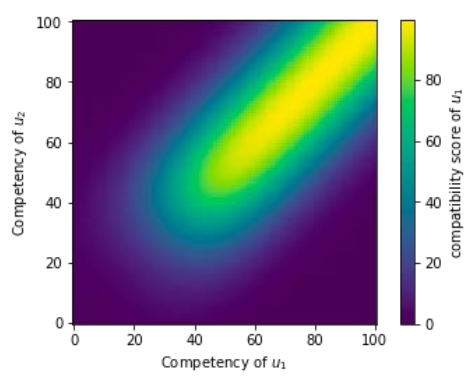
\includegraphics[width=0.5\textwidth]{g/SeekingPartnerCompatibility.PNG}
	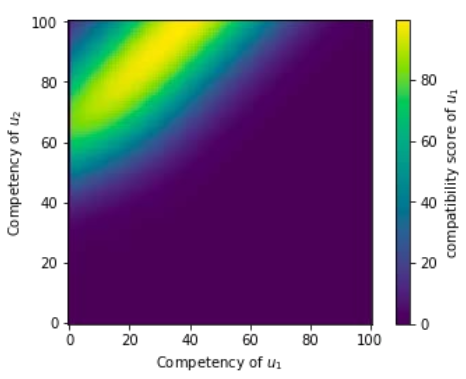
\includegraphics[width=0.5\textwidth]{g/SeekingSupportCompatibility.PNG}
	\caption{The images show the areas of compatibility of a user u2 as a function of u1's competency. Lighter areas mean high compatibility scores in accordance to u1's preferences. On the left u1 is looking for a study partner, leading to the best fit along the u1 = u2 axis. The cutoff beneath a competency of 40 is due to the minimum joint competency threshold T. On the right, we can see u1 looking for peer support, i.e. a person with considerably higher knowledge, here about 60 points higher than u1. Source: \textit{potts2018reciprocal}}
	\label{f:Seeking}
\end{figure}
In the last step, RiPPLE returns a predefined amount of matchups \(k\) with the best reciprocal values for each user. Although these reciprocal values are now symmetrical, the recommendations don't have to be: While from u1s standpoint the matchup with u2 and an (arbitrary) reciprocal score of 30 could be the very best opportunity, u2 could still have true reciprocal a matchup with u3 and a value of 50.\\
For more information on RiPPLE, the algorithm and further clarification of different variables, please reference \textit{potts2018reciprocal}.\\	
RiPPLE will be evaluated in live conditions in the course of this year. To evaluate whether the implementation could work under real conditions, Potts et al. conducted an experiment using randomly generated data.\\

\section{Evaluation}\label{paper:evaluation}
In order to test RiPPLE's applicability for actual use, Potts et al. designed an experimental setup in which RiPPLE would try to propose recommendations for randomly generated test data. Specific quality measures were designed according to \textit{olakanmi2017group} to assess different fields in which RiPPLE would have to show its capabilities. With satisfying results, RiPPLE would be able to be used under live conditions in the course of 2018.\\
To conduct the experimental evaluation, random data had to be generated; diverse enough to highlight edge cases but within reasonable bounds.\\ 
%For a set of 1000 users, 10 learning topics and 10 possible timeslots, each user received a random distribution of relevant values. Topic-specific competencies were expressed as a value from 0 to 100 derived from a truncated normal distribution around a random mean with fixed variance. Each user received competencies for every topic. These were then sorted from low to high, and a random number of these topics were chosen to be part of the user's request. The highest competencies of every user were classified as "providing support" roles, the lowest as "seeking support" and the median topic received a "co-study" role. In absence of empirical data, competency difference preferences were modeled as a fixed value per chosen role, as opposed to a explicitly stated preference for each user. Every "user" was made available during random timeslots.\\
To fully satisfy as a tool recommending students to one another, RiPPLE must be able to form meaningful and successful matches for as many users as possible in reasonable time. On the other hand, minor drawbacks in the defined metrics were considered to be tolerable in this step due to the experimental and randomly generated data and some further adjustments that could be made to compensate bad values.\\
As evaluation metrics for their experimental evaluation Potts et al. decided on four values that can further be used as general Quality Measures for reciprocal recommendation algorithms:\\

\subsection{Scalability} \label{paper:scalability}
With increasing enrollment numbers in higher education, RiPPLE will have to be suitable for large sets of learners. High runtime and costs for evaluating datasets with reasonable amounts of students means slower responses and a worse user experience. An optimal solution could provide immediate recommendations to any user, at any moment.\\
As can be seen in figure \ref{f:scalability}, the runtime of the algorithm increased in a quadratic fashion, as U, the total amount of users, increased: \(O(n^2)\). The number of recommendations per user, however, does not significantly impact the runtime. (Although the paper states that it \textit{did} in fact affect runtime, looking at the plots data suggests that this might be a formatting error.)\\
Currently, RiPPLE calculates recommendations at the end of each week for the upcoming week, making the algorithm's runtime rather unimportant. In a 1000 user experiment, RiPPLE was able to provide recommendations for a single user in 0.045 seconds. However, further improvements are planned.\\
\begin{figure}[p]
	\centering
	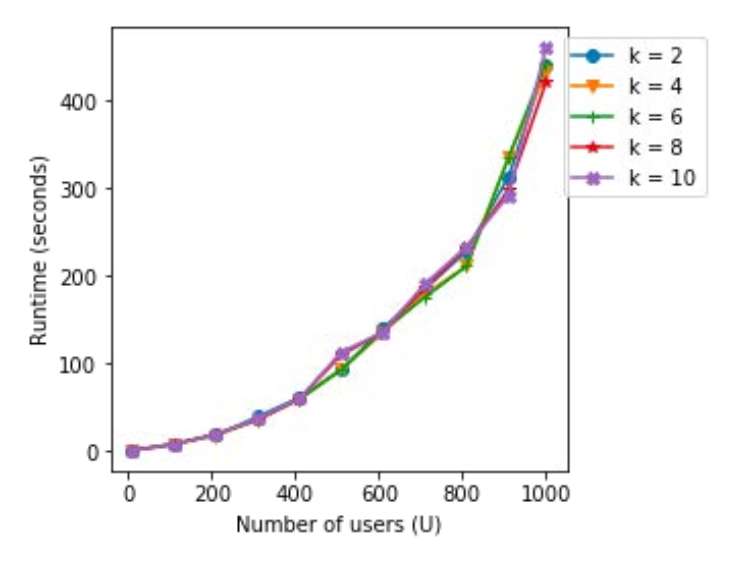
\includegraphics[width=0.5\textwidth]{g/Runtime.PNG}
	\caption{Scalability: The algorithm's runtime depending on the number of users \(U\) and the amount of recommendations per user \(k\). Note how k has almost no influence on the runtime, while it grows exponentially with increasing U. Source: \textit{potts2018reciprocal}}
	\label{f:scalability}
\end{figure}


\subsection{Reciprocality} \label{paper:reciprocality}
The best possible recommendations are reciprocal: Users contacting a recommended user would also appear on this user's list of potential study partners. \textit{prabhakar2017reciprocal} Reciprocality was tested for both, the baseline non-reciprocal and the joint reciprocal harmonic mean scores. Whenever a user appears in the recommendations of a user on their own recommendation list that was built according to the respective score, the recommendation was considered to be reciprocal.\\
The precision for every user given the used score is calculated by dividing his reciprocal recommendations through \(k\), the total amount of recommendations that user received. The system's total precision is defined as the average precision across all users. \textit{prabhakar2017reciprocal}\\ 
In all tested cases shown in figure \ref{f:reciprocality}, the reciprocal score had a higher precision than the baseline score. This is not surprising, since using the harmonic mean of both one-directional scores chooses reciprocal scores with medium values compared to non-reciprocal scores with a single high value. (As explained in section \ref{paper:Ripple}) Increasing \(k\) also increases the precision, since more recommendations per user lead to a higher chance of reciprocal recommendations. On the other hand, increasing \(U\) with a fixed \(k\) reduces reciprocal precision, since there are more possible users to recommend.\\
\begin{figure}[p]
	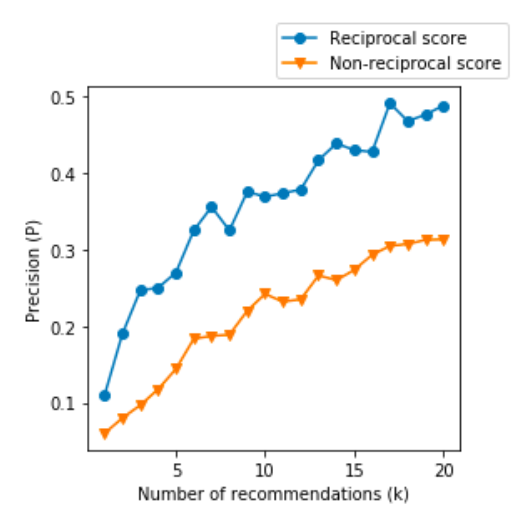
\includegraphics[width=0.5\textwidth]{g/PrecisionByK.PNG}
	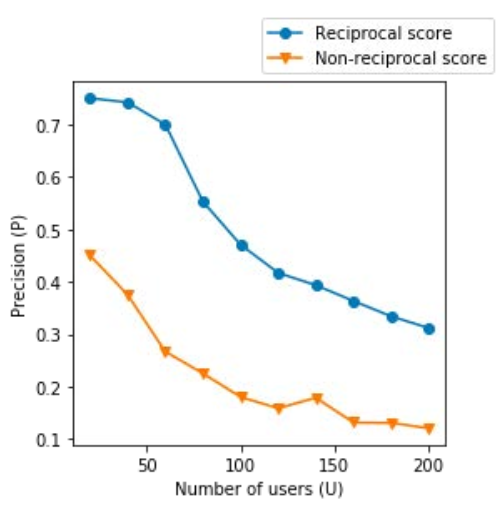
\includegraphics[width=0.5\textwidth]{g/PrecisionByU.PNG}
	\caption{Reciprocality: The precision (= the fraction of reciprocal recommendations out of the total recommendations averaged over all users) of the baseline non-reciprocal recommendations (orange) vs. of the reciprocal, averaged scores. Note how the reciprocal scores are always better. Source: \textit{potts2018reciprocal}}
	\label{f:reciprocality}
\end{figure}

\subsection{Coverage} \label{paper:coverage}
Recommending potential learning partners to one another should not abandone anyone. As such, coverage is a very important metric to consider. Since (almost) every user will receive recommendations, most users will be covered in one way or another. (The exception to this are users with completely incompatible timeslots, role preferences (i.e. being the only person looking for an equally skilled study partner) or users who can't meet the minimum competency when coupled with their available potential partners.) A very good fit can only be ensured when each user is recommended to others, ideally forming a reciprocal recommendation, which is represented in \ref{paper:reciprocality}. Coverage however is defined as the percentage of users that appear in other's recommendations at least once.\\
For a low amount of users and lots of recommendations per user, coverage is close to 0.9, meaning most users are recommended to others. As U increases or k decreases, the coverage sinks. However, more than 40\% of users appear in other's recommendations under all tested circumstances. Reference figure \ref{f:coverage} for a graphical overview.\\

\begin{figure}[p]
	\includegraphics[width=0.5\textwidth]{g/CoverageUk.PNG}
	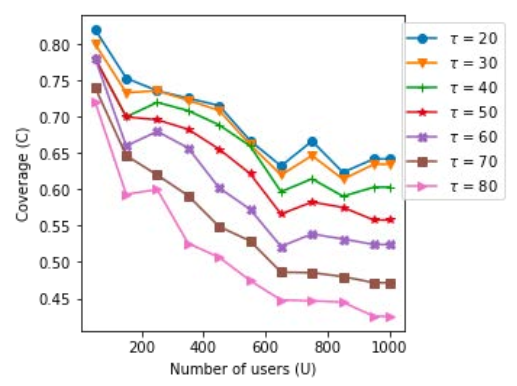
\includegraphics[width=0.5\textwidth]{g/CoverageUT.PNG}
	\caption{Coverage: The percentage of users who appear in other's recommendations. With more users, coverage sinks (likelihood of hard to match users increases). Increasing received recommendations or lowering the minimum joint competency of matches increases coverage. Mind the y-axis cutoff. Source: \textit{potts2018reciprocal}}
	\label{f:coverage}
\end{figure}

\subsection{Quality} \label{paper:quality}
The quality of a recommendation is not only based on its fit, but also on how good the resulting team could perform. According to Blumenfeld, learners should meet a minimum competency level in order to be an effective group, as specified by the employed minimum matchup threshold T. \textit{blumenfeld1996learning} Quality is thus defined as the user's average joint competencies across their matched topics. The goal is to generate matches that are as capable as possible in their respective fields of study.\\
Referencing figure \ref{f:quality}, it is apparent that the total amount of users does not affect the quality of matches. The minimum threshold for joint competency of a matchup however leads to a better quality. Comparing this finding to \ref{f:coverage} however, suggests that higher quality comes at the cost of less coverage. Especially when considering the slight improvements in quality score for larger increments in T.\\
\begin{figure}[p]
	\centering
	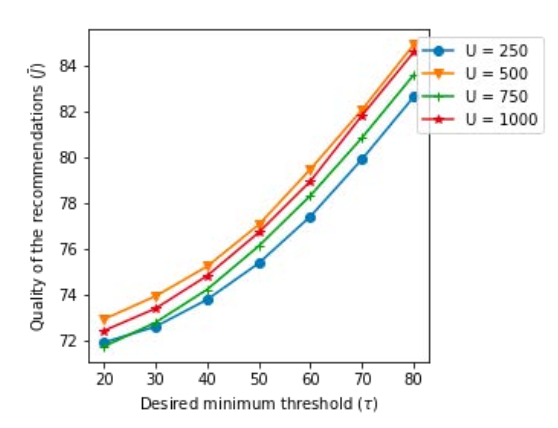
\includegraphics[width=0.5\textwidth]{g/QualityByU.PNG}
	\caption{Quality: The quality of matchups over different values for U and T. Note how changing U won't affect matchup quality. Choosing a higher minimum joint competency threshold T for successful matchups increases overall quality. Note the different scaling of the axes, overemphasizing the quality increases. Source: \textit{potts2018reciprocal}}
	\label{f:quality}
\end{figure}

\section{Discussion} \label{paper:discussion}
"Reciprocal peer recommendation for Learning Purposes" and the implemented platform RiPPLE present an approach to build a scalable, interactive and user-facing, multi-purpose learning platform to enhance learning both in on- and offline circumstances. RiPPLE's flexiblity in some threshold values allows the tool to be customised to address some of the shortcomings of peer recommender systems identified by Olakanmi and Vassileva \textit{olakanmi2017group}. While the experimental results look promising, further research on actual data has to be conducted, which is planned over the course of the year.\\
The experimental evaluation of the platform's performance using artificial data sheds light on variable relationships, potential initial values for scientifically sparse concepts and the interplay of lots of factors. While the values reported from evaluation with artificial data present good metrics to measure the algorithm's performance and suitability for live data, they don't actually evaluate the algorithm, since no target values have been set. Although the data is quantifiable, these findings should not be mistaken as quantitative results: instead of comparing the data to theory-driven goals and evaluating them for actual use, they are more or less providing an overview of how the algorithm works. In fact, there is currently no way to know if these results are "good". Some of the used measurements lack consistent data and research, and are not theoretically funded. For example, the question whether a coverage of little above 0.4 will be enough in practice, remains unanswered. Actual results from live usage are thus highly interesting and could provide insights in lots of different areas.\\
The algorithm itself does have some minor drawbacks. For one, RiPPLE calculates matchups across all topics. For example, two learners who would be a perfect match in one topic, but a bad match in another would be considered as a mediocre match. Topic-wise recommendation would further complicate the algorithm, but might lead to larger benefits for users. Another aspect are edge-cases in terms of competency preferences that would lead to overall low scores for matchups with other people, leading to learners who will receive suggestions with low scores, but won't appear in other's recommendations. While this does not necessarily lead to any consequences by itself, certain highly compatible users might be overwhelmed with meeting-requests from users outside their own recommendations. While they won't be able to meet every requesting user, these less compatible users might become abandoned.\\
Another drawback is the neglected human factor. Both user buy-in and competence in handling the tool and its demands might influence its use in practice. While this study's goal was explicitly to test the theory and future praxis tests are planned, this topic should be discussed, a major shortcoming of the paper at hand.\\
A lack in user buy-in is something that always should be considered, especially in a student context. If a student didn't want to engage with strangers, was not motivated to study with partners or to adjust his or her schedule, all recommendations to and of that student would not accomplish anything. Meeting requests would be ignored, and opportunities for matchups would expire. Even negative user manipulation needs to be considered as an possibility, but are something that has to be dealt with in the live test.\\
While missed opportunities are a problem of the students themselves, rather than of the platform providing recommendations, the other human factor needs to be addressed directly by the tool:\\
As humans are unreliable, self-reported metrics always underly lots of variance and errors. A user's competency in a specific topic, his or her preferences, or the willingness to commit to a specific timeslot for learning might change daily, dependent on mood, time of day, culture and lots of other factors. \textit{lee2002cultural} \textit{sorensen2008measuring} Other variables, like a user's preferred skill difference towards a learning partner, are especially hard to specify. How is a user supposed to know what his or her learning preferences are? How would he know which number refers to the desired difference in skill rating? From a psychological standpoint, this operationalization is bound to fail, if not controlled in an appropriate manner. \textit{gonyea2005self}\\
Delving deeper into Olakanmi and Vassilevas categorial critique of peer recommendation algorithms, we can see that Potts et al. tried to address many of their findings. \textit{olakanmi2017group} Unfortunately, some major concerns can not be covered by RiPPLE:
\begin{itemize}
	\item Usage of self-reported user preference data
	\item Inflexibility in dealing with only partially known users
	\item orphaned learners don't receive any value and have to be processed by hand
\end{itemize}
While lots of these claims do not holf for RiPPLE or could be averted by it's implementation, these findings remain problematic until disproven. \\

Taking all of this into consideration, the proposed peer learner recommendation algorithm does have its flaws but will not necessarily fail. The benefits of recommending meaningful social learning opportunities are manifold and even if RiPPLE would only be used by a fraction of the potential users, it would surely help these learners to navigate a digital world full of learning opportunities. The live test will show whether this hypothesis holds in praxis.\\


\chapter{Extensions} \label{extensions}
Choosing a user preference model that fits both the domain and the goal of an algorithm poses a major problem in peer recommendation. \textit{potts2018reciprocal, olakanmi2017group}\\
An important factor is to consider both, the information needed to create meaningful matches according to a specific success criterion, and how to access this information. Generally-speaking, automatically collected data is preferred to relieve the users as much as possible. But not all data can automatically be collected. Internal information, like preferences, date availability, motivations or the in reciprocal group formation highly important personality need to be reported by the user - there is currently no way to easily access internal information of the user's mind.\\
Psychological research was founded to enable the measurement and quanitification of these details. From psychophysical measurements to intricate operationalizations of complicated internal states, one easily accessible method stays predominant in social science: self-reported statements, from qualitative interviews to acceptance scales.\\
One such scale is the NEO-PI-R \textit{ostendorf2004neo}, arguably one of the most famous personality-measurement tools. A questionnaire with Likert-scaled \footnote{The commonly known items prompting users to reply to a statement on a scale from (usually) 1 to 5 (often combined with sentences like "I agree" or "I disagree") are called "Likert scales" after Rensis Likert. \textit{likert1932technique}} items on five axes representing the five dimensions of personality. \textit{mccrae1987validation, goldberg1990alternative}\\
While the NEO-PI-R is widely used and considered as reliable and validated, it still relies on self- or peer-reported data and can, as such, not be considered a flawless tool. For example, many self-reporting tools suffer from a relevant problem called "Faking Good", the tendency to answer items in a way that is considered to be socially acceptable. When faking good, people manipulate their answers to cohere to social norms out of fear to be seen as a bad person. It is known to influence the outcomes of some of the personality traits, measured by the NEO-PI-R.\textit{griffin2004applicants} A similar effect can be observed when peer-ratings get influenced by peer sympathy. \textit{leising2010letter}\\
In learning environments, a phenomenon known as the "Lake Wobegon Effect" influences student reports of their learning success: students tend to overstate their good performances, while failures will not be reported. This leads to an overestimation of student successes in surveys. \textit{maxwell1994lake}\\
Another example, the infamous "Likert Scale" as introduced by Rensis Likert in 1932 as an "attitude scale" \textit{likert1932technique} can safely be assumed to be one of the most used metrics in social research, while it's optimal use still remains controversial. \textit{chang1994psychometric, lee2002cultural}\\
Self-reported data still remains a largely controversal topic in psychological research: it is easy to acquire and enables researchers to access internal information, while these measurements can fluctuate following lots of different influences and are hard to validate. \textit{gonyea2005self, lee2002cultural, sorensen2008measuring}\\
Not only is a proper specification of the domain and goals of a recommender system relevant, in reciprocal recommendation, the user must be modeled as both, a recommended item and a user receiving recommendations at the same time. Modeling users however is complicated due to unreliable methods or participants (knowingly or subconsciously) manipulating their answers.\\
While Potts et al. obviously tried to choose a user-model that is limited to the necessary basics and tried to rely on as few ambigous and self-reported pieces of information as possible, they still need a user's ability in reporting information about him- or herself. (Please see section \ref{sec:disc} for a more thorough discussion of Potts et al.'s user model)\\
Other reciprocal recommendation approaches have to work around the same problems. As mentioned in section \ref{rw:reciprocalrec}, Xia et al. have shown that a behavior-emergent metric was more reliable in their use case of reciprocal online-dating recommendation. \textit{xia2014characterization} Instead of focusing on user-reported data alone, they included implicit and pre-evaluated information derived from user interactions to measure attractiveness and willingness to communicate. \textit{xia2015reciprocal} Wang et al. wanted to improve gaming matchmaking by employing problem-solving style information gathered from in-game statistics. They were able to deduce complicated, high-level cognitive problem-solving skills from simply evaluating implicit behavior, and used this information to improve player experiences. \textit{wang2015thinking}\\
Instead of asking learners for their preferences regarding the competency difference towards their peer, Potts et al. could have decided the latter themselves, founded in theory of optimal group composition. \textit{manske2015using}\\
When talking about implicit data derived from a user's interaction with the running system on the other hand, an important drawback mentioned by Olakanmi et al. needs to be considered: the cold start problem. \textit{olakanmi2017group} Relying on live data will lead to the first recommendations to be made without any underlying data, at random. Only after some burn-in, actual data can be used to achieve better results, which leads to much less acceptance for the new tool.\\

Besides building pairs of students, slightly larger groups might yield even better results. Lots of theory about group composition emphasizes the importance of different skillsets and heterogeneity. \textit{olakanmi2017group, blumenfeld1996learning, manske2015using} A system called DIANA, using a genetic framework to form small heterogenous groups in study courses used many different student characteristics to match students. An evaluation using course grades proved that this could generally be more efficient than random or self-organised group formation.\\
The gaming sector could prove to yield some interesting findings regarding group formation, since lots of factors could be considered to build a well-performing multiplayer gaming team. \textit{delalleau2012beyond, wang2015thinking, suznjevic2015application} Unfortunately, this field of study is still sparse and inconsistent itself, facing struggles like different people choosing their preferred team based on completely different strategies. \textit{riegelsberger2007personality}\\

\bibliographystyle{alpha}
\bibliography{bib}

\end{document}
